%\documentclass{beamer}
\documentclass[handout]{beamer}
\usepackage{etex}
%% % use this with the [handout] option to create handouts for the audience
% \usepackage{pgfpages}
% \pgfpagesuselayout{2 on 1}[a4paper,border shrink=5mm]

\mode<presentation>
{
  \usetheme{Diku}
  % set this to your preferences:
  \setbeamercovered{invisible}
  %\setbeamercovered{transparent}
}
\usepackage{listings}
\usepackage{framed}
\usepackage{graphicx}
\usepackage{adjustbox}
\usepackage{epic}
\usepackage{url}
\usepackage{paratype}
\usepackage{xcolor}
\usepackage{ulem}
\usepackage{multirow}
\usepackage[utf8]{inputenc}
\usepackage{caption}
\usepackage{mathrsfs}
\setbeamerfont{frametitle}{family=\bf}


\setbeamertemplate{bibliography item}{\insertbiblabel}

\usepackage{amsmath}
\usepackage{amssymb}
\usepackage{amsthm}

\newcommand{\basetop}[1]{\vtop{\vskip-1ex\hbox{#1}}}
\newcommand{\source}[1]{\let\thefootnote\relax\footnotetext{\scriptsize\textcolor{kugray1}{Source: #1}}}
\definecolor{mygreen}{RGB}{50, 96, 60}

\lstdefinelanguage{Futhark}
{keywords={fun,if,then,else,loop,do,map,reduce,filter,scan,redomap,transpose,reshape,iota,replicate,let,in,for,while,with,f32,int,zip,streamRed,zipWith, unsafe},%
  sensitive=true,%
  comment=[l]{--},%
  string=[b]",%
  moredelim=**[is][\color{red}]{@}{@},
  moredelim=**[is][\color{blue}]{¤}{¤},
}

\lstset{
  language=Futhark,
  basicstyle=\footnotesize
}

% for coloured code citation in text:
\usepackage{fancyvrb}

%%%%%%%%%%%%%%%%%%%%%%%%%%%%%%%%%
%%%%% code sections   %%%%%%%%
%%%%%%%%%%%%%%%%%%%%%%%%%%%%%%%%%

% code highlighting commands in own block
\DefineVerbatimEnvironment{code}{BVerbatim}{}
\DefineVerbatimEnvironment{icode}{Verbatim}{fontsize=\scriptsize}
\DefineVerbatimEnvironment{tinycode}{Verbatim}{fontsize=\tiny}

% Fancy code with color commands:
\DefineVerbatimEnvironment{colorcode}%
{Verbatim}{fontsize=\scriptsize,commandchars=\\\{\}}
\DefineVerbatimEnvironment{smallcode}%
{Verbatim}{fontsize=\tiny,commandchars=\\\{\}}

%%%%%%%%%%%%%%%%%%%%%%%%%%%%%%%%%%
%%%%% some coloring    %%%%%%%%

% use "DIKU green" from our color theme for \emph
\renewcommand{\emph}[1]{\textcolor{structure}{#1}}
% use some not-too-bright red for an \emp command
\definecolor{DikuRed}{RGB}{130,50,32}
\newcommand{\emp}[1]{\textcolor{DikuRed}{ #1}}
\definecolor{CosGreen}{RGB}{10,100,70}
\newcommand{\emphh}[1]{\textcolor{CosGreen}{ #1}}
\definecolor{CosBlue}{RGB}{55,111,122}
\newcommand{\emphb}[1]{\textcolor{CosBlue}{ #1}}
\definecolor{CosRed}{RGB}{253,1,1}
\newcommand{\empr}[1]{\textcolor{CosRed}{ #1}}

\newcommand{\mymath}[1]{$ #1 $}
\newcommand{\myindx}[1]{_{#1}}
\newcommand{\myindu}[1]{^{#1}}

\newcommand{\myalt}{~|~}

\makeatletter
\long\def\beamer@author[#1]#2{%
  \def\insertauthor{\def\inst{\beamer@insttitle}\def\and{\beamer@andtitle}%
    \begin{tabular}{lr}#2\end{tabular}}%
  \def\beamer@shortauthor{#1}%
  \ifbeamer@autopdfinfo%
  \def\beamer@andstripped{}%
  \beamer@stripands#1 \and\relax
  {\let\inst=\@gobble\let\thanks=\@gobble\def\and{, }\hypersetup{pdfauthor={\beamer@andstripped}}}
  \fi%
}
\makeatother

%%%%%%%%%%%%%%%%%%%%

\title{Programming Massively Parallel Hardware\\\textbf{Simplex on the GPU}}

\author[]{%
  Anders Wind Steffensen \\
  Chi Pham \\
  Michael Hejselbak Jensen \\
}

\institute{Department of Computer Science (DIKU)\\University of Copenhagen}


\date[3/3]{November 9th 2017}


\begin{document}

\titleslide

%%%%%%%%%%%%%%%%%%%%%%%%%%%%%%%%%%%%%%%%%%%%%%%%%%%%%%%%%%%%%%%%%%%%%%

\begin{frame}
  \frametitle{Overview}
  \begin{itemize}
  \item Introduction
  \item Design
  \item Implementation
  \item Design
  \item Results
  \item Conclusion
  \end{itemize}
\end{frame}

%%%%%%%%%%%%%%
% INTRO
%%%%%%%%%%%%%%

\begin{frame}[fragile]
\frametitle{Futhark test}
Futhark test
\pause
\begin{lstlisting}
// @emphasis@
// ¤emphasis2¤
let simplex [n] [m] (A : [m][n]f32) (b : [m]f32)
  (c : [n]f32) (v : f32) =
  let e = entering_variable c
  let (_,_,_,v,_) = loop (A,b,c,v,e) while e != -1 do
    let l = leaving_variable A b e
    let (A,b,c,v) = unsafe pivot A b c v l e
    let e = entering_variable c
    in (A,b,c,v,e)
  in v

\end{lstlisting}
\end{frame}

%%%%%%%%%%%%%%
% DESIGN
%%%%%%%%%%%%%%

\begin{frame}
The three flattened versions.
\begin{itemize}
	\item \textbf{Outer parallel}: Instances are computed in parallel. Simplex is not parallelized. Flattening is not needed.
	
	\item \textbf{Inner parallel}: Simplex is computed in parallel. Not parallel across instances. Small degree of flattening.
	
	\item \textbf{Fully parallel}: Simplex and instances are computed in parallel. High degree of flattening.
\end{itemize}
\end{frame}

%%%%%%%%%%%%%%
% IMPLEMENTATION
%%%%%%%%%%%%%%

%%%%%%%%%%%%%%
% RESULTS
%%%%%%%%%%%%%%
\begin{frame}[fragile]
\frametitle{One Big Instance}
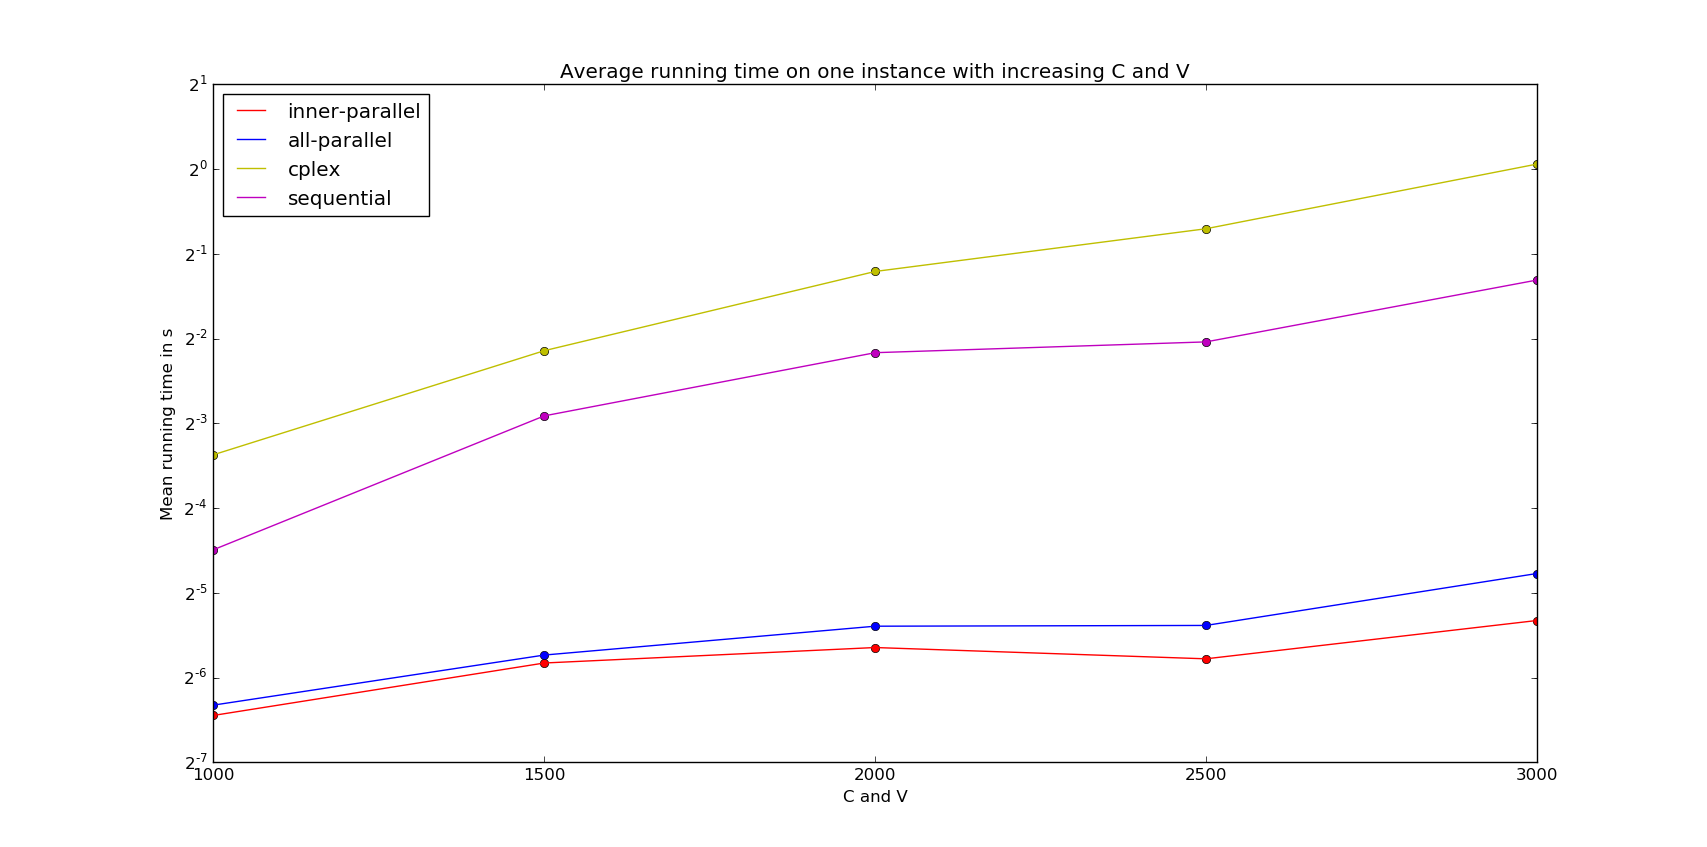
\includegraphics[width=\textwidth]{../Doc/figures/one-big}
\end{frame}

\begin{frame}[fragile]
\frametitle{Many Small Instance}
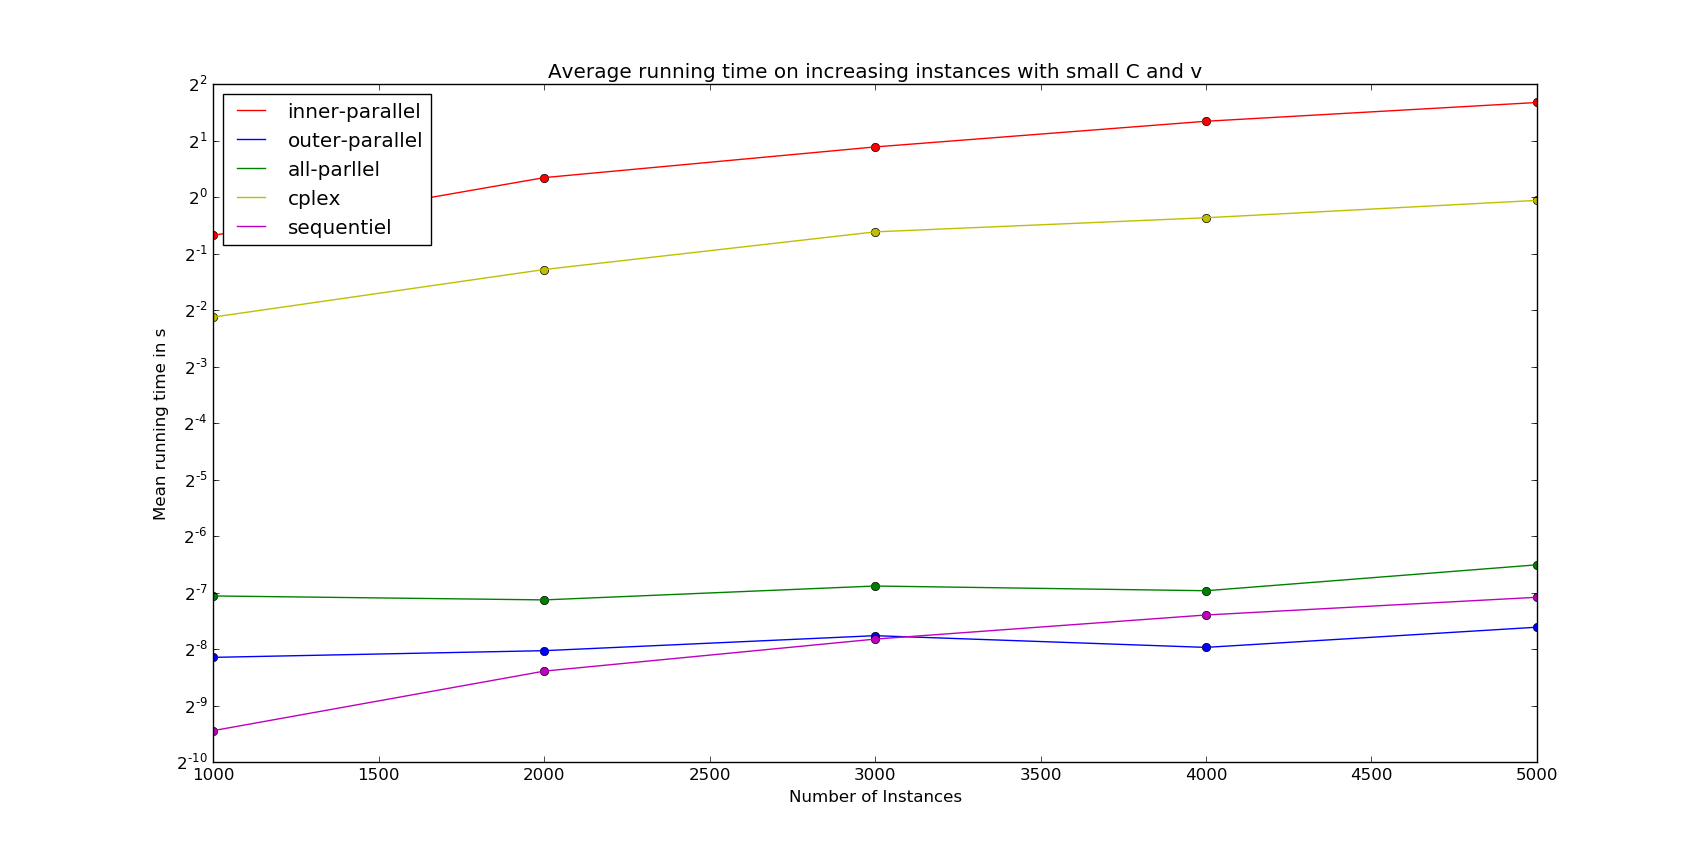
\includegraphics[width=\textwidth]{../Doc/figures/many-small}
\end{frame}

\begin{frame}[fragile]
\frametitle{Many Instance of Varying Size}
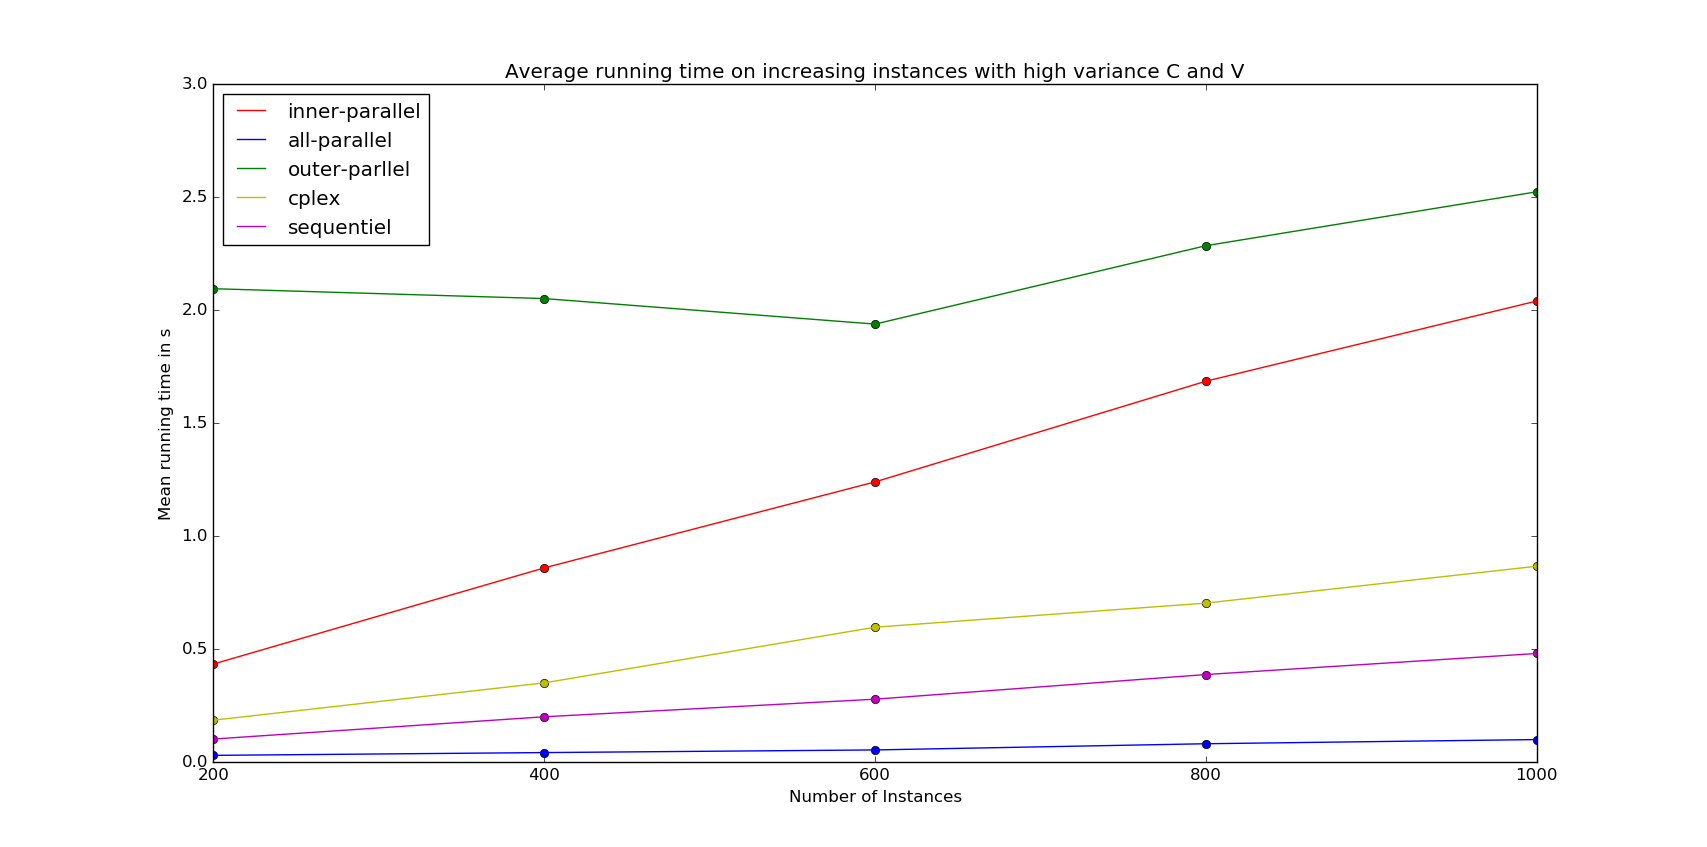
\includegraphics[width=\textwidth]{../Doc/figures/many-varying}
\end{frame}

\begin{frame}[fragile]
\frametitle{Many Big Instance}
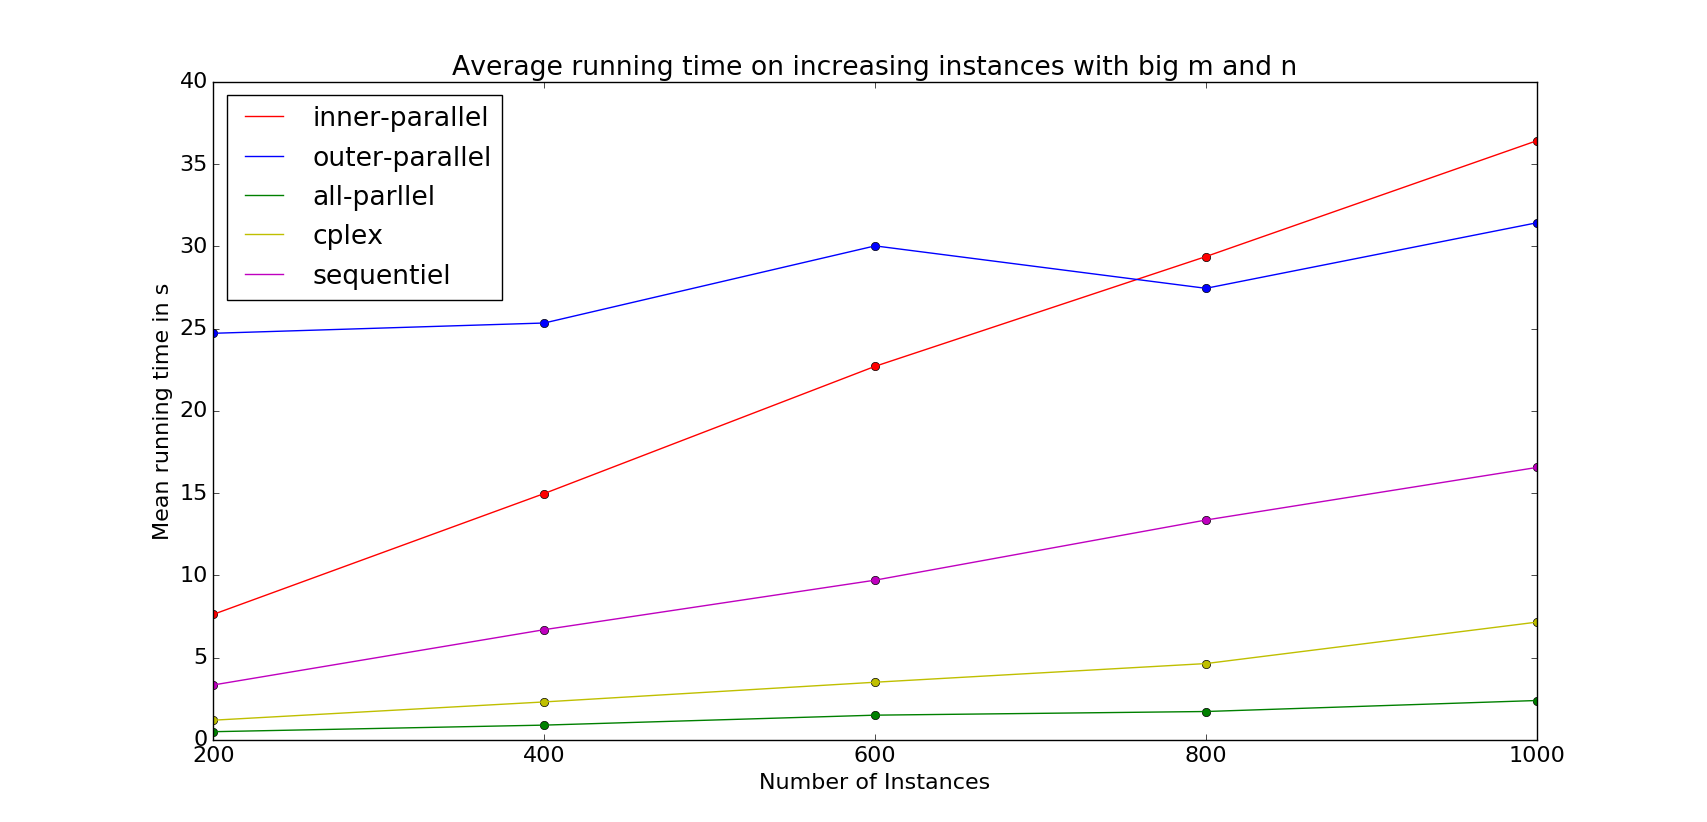
\includegraphics[width=\textwidth]{../Doc/figures/many-big}
\end{frame}

\begin{frame}
\frametitle{Number of pivots for the biggest test sets}
\textbf{Many small instances, M and N between 1 and 10}\\ mean is: 3.772, standard deviation is: 2.630\\
\textbf{Many varying instances, M and N between 10 and 150}\\ mean is: 77.192, standard deviation is: 53.616\\
\textbf{Many big instances, M and N between 150 and 200}\\ mean is: 254.283, standard deviation is: 79.926
\end{frame}
%%%%%%%%%%%%%%
% CONCLUSION
%%%%%%%%%%%%%%

\end{document}

%%% Local Variables:
%%% mode: latex
%%% TeX-master: t
%%% End:
